\documentclass[12pt, twoside]{article}
% Full article preamble (duplicated, no common file)
\usepackage{fontspec}
\usepackage[a4paper,margin=2.5cm,includefoot]{geometry}
\usepackage{polyglossia}
\usepackage{amsmath}
\usepackage{amssymb}
\usepackage{xcolor}
\usepackage{fancyhdr}
\usepackage{graphicx}
\usepackage{listings}
\usepackage[most]{tcolorbox}
\usepackage{pifont}
\usepackage{enumitem}
\usepackage{titlesec}
\usepackage[bottom]{footmisc}
\usepackage{titling}
\usepackage{minted}
\usepackage{etoolbox}
\usepackage{array}
\usepackage{extsizes}

\newfontfamily\emoji{Segoe UI Emoji}

\pagestyle{fancy}

\setmainlanguage[numerals=western]{arabic}
\setotherlanguage{english}
\newfontfamily\arabicfont[Script=Arabic]{Amiri}
\newfontfamily\arabicfonttt[Script=Arabic]{Courier New}

\lstset{
  language=[Sharp]C,
  numbers=left,
  stepnumber=1,
  numbersep=8pt,
  frame=single,
  basicstyle=\ttfamily\small,
  keywordstyle=\color{blue},
  stringstyle=\color{red},
  commentstyle=\color{green!50!black}
}

\newif\ifdetailed
\ifdefined\setdetailed
  \setdetailed
\fi

\newif\ifwithsols
\ifdefined\setwithsols
  \setwithsols
\fi

% unified tcolorboxes for articles
\tcbset{colback=white, colframe=black, fonttitle=\bfseries, boxrule=0.8pt}
\newtcolorbox{boxDef}[1][]{colback=blue!5!white,colframe=blue!75!black,
  title={{\emoji📘} تعريف\ifx\\#1\\\else ~#1\fi :}}
\newtcolorbox{boxExercise}[1][]{colback=cyan!5!white,colframe=cyan!70!black,
  title={{\emoji🧩} تمرين\ifx\\#1\\\else ~#1\fi :}}
\newtcolorbox{boxExample}[1][]{colback=yellow!5!white,colframe=orange!90!black,
  title={{\emoji📝} مثال\ifx\\#1\\\else ~#1\fi :}}
\newtcolorbox{boxNote}[1][]{colback=gray!10!white,colframe=black,
  title={{\emoji✨} ملاحظة\ifx\\#1\\\else ~#1\fi :}}
\newtcolorbox{boxAttention}[1][]{colback=magenta!10!white,colframe=magenta!80!black,
  title={{\emoji🔔} تنبيه\ifx\\#1\\\else ~#1\fi :}}
\newtcolorbox{boxWarning}[1][]{colback=red!5!white,colframe=red!75!black,
  title={{\emoji⚡} ملاحظة هامة\ifx\\#1\\\else ~#1\fi :}}
\newtcolorbox{boxSolution}[1][]{colback=green!5!white,colframe=green!60!black,
  title={{\emoji✅} حل\ifx\\#1\\\else ~#1\fi :}}
\newtcolorbox{boxSymbol}[1][]{colback=purple!5!white,colframe=purple!70!black,
  title={{\emoji🔣} رمز\ifx\\#1\\\else ~#1\fi :}}

\tcbset{simplecode/.style={ colback=gray!5, colframe=black!50, boxrule=0.4pt, arc=2pt, left=4pt,right=4pt,top=4pt,bottom=4pt}}
\newenvironment{boxCode}{\begin{tcolorbox}[simplecode]}{\end{tcolorbox}}

\newcolumntype{C}[1]{>{\centering\arraybackslash}p{#1}}

% redefine spaces after titles
\makeatletter
\renewcommand{\@maketitle}{%
  \begin{center}
    {\huge \bfseries \@title \par}%
    \vskip 0.2em % space between title and author
    {\large \@author \par}%
    % \vskip 0.2em % space between author and date
    % {\normalsize \@date \par}%
  \end{center}
}
\makeatother

\fancyhf{} % clear default
\fancypagestyle{plain}{
  \fancyhf{}
  \fancyhead[L]{مدرسة التسامح الشاملة}
  % \fancyhead[L]{
\includegraphics[height=1cm]{../../../images/logoTasamoh.png}}
  \fancyhead[R]{الأستاذ محمود اغبارية}
  \fancyfoot[C]{\thepage}
}

\fancyhead[L]{مدرسة التسامح الشاملة}
\fancyhead[R]{الأستاذ محمود اغبارية}
\fancyfoot[C]{\thepage}
% \date{\today}

\setcounter{tocdepth}{3} % only section subsection and subsubsection in TOC


% ----------------------


% \begin{document}

% \maketitle

% % \clearpage  % start TOC on a new page
% % \renewcommand{\contentsname}{جدول المحتويات}
% % \tableofcontents
% % \clearpage

% \part*{part 1} % the * prevents numbering
% \section*{مقدمة}
% \subsection*{مثال رياضي}
% \subsubsection*{مثال فرعي}
% \paragraph*{ paragraph 1}
% \subparagraph*{sub paragraph 1}

% \ifdetailed
% \begin{english}
% \begin{minted}{csharp}
% // C# Example
% \end{minted}
% \end{english}
% \fi

% OLD WAY
% \ifdetailed
% \begin{english}
% \begin{lstlisting}
% // C# Example
% \end{lstlisting}
% \end{english}
% \fi

% % 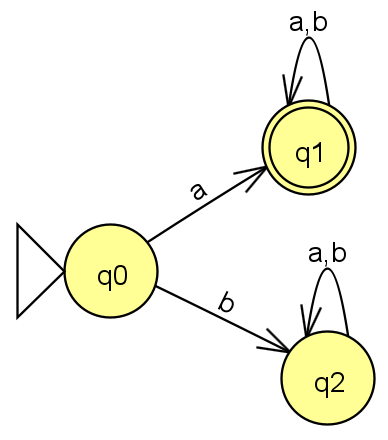
\includegraphics[width=0.2\textwidth]{../../../images/DFAs/ex1_q1.png}



% \vspace{3cm}
% \begin{flushleft}
% أرجو لكم وقتًا ممتعًا.

% الأستاذ محمود اغبارية.
% \end{flushleft}


% \end{document}


\title{ورقة تمرن 4 للصف العاشر 10 $\mathtt{if\ Statement}$}

\begin{document}

\maketitle
\thispagestyle{fancy}

\ifdetailed
\begin{enumerate}[itemsep=3em]
\else
\begin{enumerate}
\fi


\item
اكتب برنامجًا يستقبل من المستخدم درجة حرارة، ويطبع له "\textbf{الجو حار}" إذا كانت درجة الحرارة أكثر من 30 درجة.
\ifdetailed
\begin{boxExample}[1]
\begin{english}
\begin{minted}{text}
Enter temperature:
35
It's hot
\end{minted}
\end{english}
\end{boxExample}

\begin{boxExample}[2]
\begin{english}
\begin{minted}{text}
Enter temperature:
25
\end{minted}
\end{english}
\end{boxExample}

\ifwithsols
\begin{boxSolution}
\begin{english}
\begin{minted}{csharp}
private static void Main(string[] args)
{
    Console.WriteLine("Enter temperature:");
    int temperature = int.Parse(Console.ReadLine());
    if (temperature > 30)
    {
        Console.WriteLine("It's hot");
    }
}
\end{minted}
\end{english}
\end{boxSolution}
\clearpage
\fi
\fi

\item
اكتب برنامجًا يستقبل من المستخدم رقمين، ويطبع له "\textbf{الرقم الأول أكبر}" إذا كان الرقم الأول أكبر من الثاني، و"\textbf{الرقم الثاني أكبر}" إذا كان الرقم الثاني أكبر من الأول.
\ifdetailed
\begin{boxExample}[1]
\begin{english}
\begin{minted}{text}
Enter first number:
15
Enter second number:
10
The first number is larger
\end{minted}
\end{english}
\end{boxExample}
\begin{boxExample}[2]
\begin{english}
\begin{minted}{text}
Enter first number:
5
Enter second number:
12
The second number is larger
\end{minted}
\end{english}
\end{boxExample}

\ifwithsols
\begin{boxSolution}
\begin{english}
\begin{minted}{csharp}
private static void Main(string[] args)
{
    Console.WriteLine("Enter first number:");
    int num1 = int.Parse(Console.ReadLine());
    Console.WriteLine("Enter second number:");
    int num2 = int.Parse(Console.ReadLine());
    if (num1 > num2)
    {
        Console.WriteLine("The first number is larger");
    }
    else
    {
        Console.WriteLine("The second number is larger");
    }
}
\end{minted}
\end{english}
\end{boxSolution}
\fi
\clearpage
\fi

\item
اكتب برنامجًا يستقبل من المستخدم رقمين، ويطبع له "\textbf{لهما نفس الإشارة}" إذا كان كلاهما موجبَين أو كلاهما سالبين، و"\textbf{إشارتان مختلفتان}" إذا كان أحدهما موجبًا والآخر سالبًا.
(افترض أنّ الرقمين ليسا صفرًا.)
\ifdetailed
\begin{boxExample}[1]
\begin{english}
\begin{minted}{text}
Enter first number:
5
Enter second number:
-3
Different signs
\end{minted}
\end{english}
\end{boxExample}
\begin{boxExample}[2]
\begin{english}
\begin{minted}{text}
Enter first number:
-4
Enter second number:
-7
Same sign
\end{minted}
\end{english}
\end{boxExample}

\ifwithsols
\begin{boxSolution}
\begin{english}
\begin{minted}{csharp}
Console.WriteLine("Enter first number:");
int num1 = int.Parse(Console.ReadLine());
Console.WriteLine("Enter second number:");
int num2 = int.Parse(Console.ReadLine());

int product = num1 * num2;
if (product > 0)
{
    Console.WriteLine("Same sign");
}
else
{
    Console.WriteLine("Different signs");
}
\end{minted}
\end{english}
\end{boxSolution}
\fi
\clearpage
\fi

\item اكتب برنامجًا يستقبل من المستخدم عددًا صحيحا، ويطبع له رسالة مناسبة عن العدد: هل الرقم مكون من منزلة، أو منزلتين، أو أكثر.
\ifdetailed
\begin{boxExample}[1]
\begin{english}
\begin{minted}{text}
Enter number:
1234
The number is made of more than 2 digits.
\end{minted}
\end{english}
\end{boxExample}
\begin{boxExample}[2]
\begin{english}
\begin{minted}{text}
Enter number:
12
The number is made of 2 digits
\end{minted}
\end{english}
\end{boxExample}
\begin{boxExample}[3]
\begin{english}
\begin{minted}{text}
Enter number:
1
The number is made of one digit
\end{minted}
\end{english}
\end{boxExample}

\ifwithsols
\begin{boxSolution}
\begin{english}
\begin{minted}{csharp}
private static void Main(string[] args)
{
    Console.WriteLine("Enter number:");
    int num = int.Parse(Console.ReadLine());
    if (n < 10)
    {
        Console.WriteLine("One digit");
    }
    else if (n < 100)
    {
        Console.WriteLine("Two digits");
    }
    else
    {
        Console.WriteLine("Many digits");
    }
}
\end{minted}
\end{english}
\end{boxSolution}
\fi
\clearpage
\fi

\item
اكتب برنامجًا يستقبل من المستخدم علامة طالب، ويطبع له التقدير المناسب حسب العلامة:
\begin{itemize}
\item \texttt{A+} إذا كانت العلامة 95 أو أكثر
\item \texttt{A} إذا كانت العلامة 90-94
\item \texttt{A-} إذا كانت العلامة 85-89
\item \texttt{B+} إذا كانت العلامة 80-84
\item \texttt{B} إذا كانت العلامة 75-79
\item \texttt{B-} إذا كانت العلامة 70-74
\item \texttt{C} إذا كانت العلامة أقل من 70
\end{itemize}%
\ifdetailed
\begin{boxExample}[1]
\begin{english}
\begin{minted}{csharp}
Enter your grade:
97
A+
\end{minted}
\end{english}
\end{boxExample}
\begin{boxExample}[2]
\begin{english}
\begin{minted}{csharp}
Enter your grade:
82
B+
\end{minted}
\end{english}
\end{boxExample}
\begin{boxExample}[3]
\begin{english}
\begin{minted}{csharp}
Enter your grade:
65
C
\end{minted}
\end{english}
\end{boxExample}

\ifwithsols
\begin{boxSolution}
\begin{english}
\begin{minted}{csharp}
private static void Main(string[] args)
{
    Console.WriteLine("Enter your grade:");
    int grade = int.Parse(Console.ReadLine());
    if (grade >= 95)
    {
        Console.WriteLine("A+");
    }
    else if (grade >= 90)
    {
        Console.WriteLine("A");
    }
    else if (grade >= 85)
    {
        Console.WriteLine("A-");
    }
    else if (grade >= 80)
    {
        Console.WriteLine("B+");
    }
    else if (grade >= 75)
    {
        Console.WriteLine("B");
    }
    else if (grade >= 70)
    {
        Console.WriteLine("B-");
    }
    else
    {
        Console.WriteLine("C");
    }
}
\end{minted}
\end{english}
\end{boxSolution}
\clearpage
\fi
\fi

\item اكتب برنامجًا يستقبل من المستخدم 3 أعداد صحيحة، ويطبعها مرتّبة من الصغير إلى الكبير.

\ifdetailed
\ifwithsols
\begin{boxSolution}
\begin{english}
\begin{minted}{csharp}
private static void Main(string[] args)
{
    Console.WriteLine("Enter three numbers:");
    int a = int.Parse(Console.ReadLine());
    int b = int.Parse(Console.ReadLine());
    int c = int.Parse(Console.ReadLine());
    if(a > b && a > c)
    {
        if (b > c)
        {
        Console.WriteLine(c + "<" + b + "<" + a);
        }
        else
        {
            Console.WriteLine(b + "<" + c + "<" + a);
        }
    }
    else if(b > a && b > c)
    {
        if (a > c)
        {
        Console.WriteLine(c + "<" + a + "<" + b);
        }
        else
        {
            Console.WriteLine(a + "<" + c + "<" + b);
        }
    }
    else // c > a && c > b
    {
        if (a > b)
        {
        Console.WriteLine(b + "<" + a + "<" + c);
        }
        else
        {
            Console.WriteLine(a + "<" + b + "<" + c);
        }
    }
}
\end{minted}
\end{english}
\end{boxSolution}
\fi
\clearpage
\fi

\item
اكتب برنامجًا يستقبل من المستخدم عمر شخص ودرجة حرارة، ويطبع له "\textbf{يمكنك الخروج}" إذا كان عمره 18 أو أكثر ودرجة الحرارة أقل من 35.
\ifdetailed
\begin{boxExample}[1]
\begin{english}
\begin{minted}{text}
Enter your age:
20
Enter temperature:
30
You can go out
\end{minted}
\end{english}
\end{boxExample}
\begin{boxExample}[2]
\begin{english}
\begin{minted}{text}
Enter your age:
16
Enter temperature:
30
\end{minted}
\end{english}
\end{boxExample}

\ifwithsols
\begin{boxSolution}
\begin{english}
\begin{minted}{csharp}
private static void Main(string[] args)
{
    Console.WriteLine("Enter your age:");
    int age = int.Parse(Console.ReadLine());
    Console.WriteLine("Enter temperature:");
    int temperature = int.Parse(Console.ReadLine());

    if (age >= 18 && temperature < 35)
    {
        Console.WriteLine("You can go out");
    }
}
\end{minted}
\end{english}
\end{boxSolution}
\clearpage
\fi
\fi

\item
اكتب برنامجًا يستقبل من المستخدم رقمين، ويطبع له "\textbf{الرقمان موجبان}" إذا كان كلاهما أكبر من صفر.
\ifdetailed
\begin{boxExample}[1]
\begin{english}
\begin{minted}{text}
Enter first number:
5
Enter second number:
8
Both numbers are positive
\end{minted}
\end{english}
\end{boxExample}
\begin{boxExample}[2]
\begin{english}
\begin{minted}{text}
Enter first number:
-3
Enter second number:
7
\end{minted}
\end{english}
\end{boxExample}

\ifwithsols
\begin{boxSolution}
\begin{english}
\begin{minted}{csharp}
private static void Main(string[] args)
{
    Console.WriteLine("Enter first number:");
    int num1 = int.Parse(Console.ReadLine());
    Console.WriteLine("Enter second number:");
    int num2 = int.Parse(Console.ReadLine());

    if (num1 > 0 && num2 > 0)
    {
        Console.WriteLine("Both numbers are positive");
    }
}
\end{minted}
\end{english}
\end{boxSolution}
\fi
\clearpage
\fi

\item
اكتب برنامجًا يستقبل من المستخدم درجة حرارة، ويطبع له "\textbf{الجو غير مناسب}" إذا كانت درجة الحرارة أقل من 10 أو أكثر من 40.
\ifdetailed
\begin{boxExample}[1]
\begin{english}
\begin{minted}{text}
Enter temperature:
5
Weather is not suitable
\end{minted}
\end{english}
\end{boxExample}
\begin{boxExample}[2]
\begin{english}
\begin{minted}{text}
Enter temperature:
25
\end{minted}
\end{english}
\end{boxExample}

\ifwithsols
\begin{boxSolution}
\begin{english}
\begin{minted}{csharp}
private static void Main(string[] args)
{
    Console.WriteLine("Enter temperature:");
    int temperature = int.Parse(Console.ReadLine());

    if (temperature < 10 || temperature > 40)
    {
        Console.WriteLine("Weather is not suitable");
    }
}
\end{minted}
\end{english}
\end{boxSolution}
\clearpage
\fi
\fi

\item
اكتب برنامجًا يستقبل من المستخدم نوع اليوم (1 للعمل، 2 للعطلة) ودرجة الحرارة، ويطبع له "\textbf{يوم ممتع}" إذا كان يوم عطلة أو درجة الحرارة بين 20 و 25.
\ifdetailed
\begin{boxExample}[1]
\begin{english}
\begin{minted}{text}
Enter day type (1=Work, 2=Holiday):
2
Enter temperature:
30
Enjoyable day
\end{minted}
\end{english}
\end{boxExample}
\begin{boxExample}[2]
\begin{english}
\begin{minted}{text}
Enter day type (1=Work, 2=Holiday):
1
Enter temperature:
22
Enjoyable day
\end{minted}
\end{english}
\end{boxExample}

\ifwithsols
\begin{boxSolution}
\begin{english}
\begin{minted}{csharp}
private static void Main(string[] args)
{
    Console.WriteLine("Enter day type (1=Work, 2=Holiday):");
    int dayType = int.Parse(Console.ReadLine());
    Console.WriteLine("Enter temperature:");
    int temperature = int.Parse(Console.ReadLine());

    if (dayType == 2 || (temperature >= 20 && temperature <= 25))
    {
        Console.WriteLine("Enjoyable day");
    }
}
\end{minted}
\end{english}
\end{boxSolution}
\fi
\clearpage
\fi

\item
اكتب برنامجًا يستقبل من المستخدم رقم، ويطبع له "\textbf{الرقم ليس صفر}" إذا كان الرقم لا يساوي صفر.
\ifdetailed
\begin{boxExample}[1]
\begin{english}
\begin{minted}{text}
Enter a number:
5
The number is not zero
\end{minted}
\end{english}
\end{boxExample}
\begin{boxExample}[2]
\begin{english}
\begin{minted}{text}
Enter a number:
0
\end{minted}
\end{english}
\end{boxExample}

\ifwithsols
\begin{boxSolution}
\begin{english}
\begin{minted}{csharp}
private static void Main(string[] args)
{
    Console.WriteLine("Enter a number:");
    int number = int.Parse(Console.ReadLine());

    if (!(number == 0))
    {
        Console.WriteLine("The number is not zero");
    }
}
\end{minted}
\end{english}
\end{boxSolution}
\clearpage
\fi
\fi

\item
اكتب برنامجًا يستقبل من المستخدم رقمين، ويطبع له "\textbf{الرقمان غير متساويين}" إذا كان الرقم الأول لا يساوي الثاني.
\ifdetailed
\begin{boxExample}[1]
\begin{english}
\begin{minted}{text}
Enter first number:
5
Enter second number:
8
The numbers are not equal
\end{minted}
\end{english}
\end{boxExample}
\begin{boxExample}[2]
\begin{english}
\begin{minted}{text}
Enter first number:
7
Enter second number:
7
\end{minted}
\end{english}
\end{boxExample}

\ifwithsols
\begin{boxSolution}
\begin{english}
\begin{minted}{csharp}
private static void Main(string[] args)
{
    Console.WriteLine("Enter first number:");
    int num1 = int.Parse(Console.ReadLine());
    Console.WriteLine("Enter second number:");
    int num2 = int.Parse(Console.ReadLine());

    if (!(num1 == num2))
    {
        Console.WriteLine("The numbers are not equal");
    }
}
\end{minted}
\end{english}
\end{boxSolution}
\fi
\clearpage
\fi

\item
اكتب برنامجًا يستقبل من المستخدم نوع الحيوان \texttt{1} للقط، \texttt{2} للكلب وعمره بالأشهر، ويطبع له رسالة مناسبة:
\begin{itemize}
\item إذا كان قط وعمره 12 شهر أو أكثر: "\textbf{قط بالغ}"
\item إذا كان قط وعمره أقل من 12 شهر: "\textbf{قط صغير}"
\item إذا كان كلب وعمره 12 شهر أو أكثر: "\textbf{كلب بالغ}"
\item إذا كان كلب وعمره أقل من 12 شهر: "\textbf{كلب صغير}"
\end{itemize}%
\ifdetailed
\begin{boxExample}[1]
\begin{english}
\begin{minted}{text}
Enter animal type (1=Cat, 1=Dog):
1
Enter age in months:
18
Adult cat
\end{minted}
\end{english}
\end{boxExample}
\begin{boxExample}[2]
\begin{english}
\begin{minted}{text}
Enter animal type (1=Cat, 2=Dog):
2
Enter age in months:
8
Young dog
\end{minted}
\end{english}
\end{boxExample}

\ifwithsols
\begin{boxSolution}
\begin{english}
\begin{minted}{csharp}
private static void Main(string[] args)
{
    Console.WriteLine("Enter animal type (1=Cat, 2=Dog):");
    int animalType = int.Parse(Console.ReadLine());
    Console.WriteLine("Enter age in months:");
    int age = int.Parse(Console.ReadLine());

    if (animalType == 1)
    {
        if (age >= 12)
        {
            Console.WriteLine("Adult cat");
        }
        else
        {
            Console.WriteLine("Young cat");
        }
    }
    else
    {
        if (age >= 12)
        {
            Console.WriteLine("Adult dog");
        }
        else
        {
            Console.WriteLine("Young dog");
        }
    }
}
\end{minted}
\end{english}
\end{boxSolution}
\fi
\clearpage
\fi

\item
معطى:
\begin{itemize}
\item متوسط درجة الحرارة في الشتاء: 15 درجة
\item متوسط درجة الحرارة في الصيف: 30 درجة
\end{itemize}%
اكتب برنامجًا يستقبل من المستخدم درجة الحرارة والفصل (1 للشتاء، 2 للصيف)، ويطبع له رسالة مناسبة:
\begin{itemize}
\item إذا كانت درجة الحرارة أعلى من المتوسط في الفصل الذي أدخله المستخدم فإنّه يطبع: \\ "\textbf{حار [اسم الفصل]}"
\item إذا كانت درجة الحرارة أقل من أو تساوي المتوسط في الفصل الذي أدخله المستخدم فإنّه يطبع: \\ "\textbf{برد [اسم الفصل]}"
\end{itemize}%
\ifdetailed
\begin{boxExample}[1]
\begin{english}
\begin{minted}{text}
Enter temperature:
20
Enter season (1=Winter, 2=Summer):
1
Hot Winter
\end{minted}
\end{english}
\end{boxExample}
\begin{boxExample}[2]
\begin{english}
\begin{minted}{text}
Enter temperature:
25
Enter season (1=Winter, 2=Summer):
2
Cold Summer
\end{minted}
\end{english}
\end{boxExample}

\ifwithsols
\begin{boxSolution}
\begin{english}
\begin{minted}{csharp}
private static void Main(string[] args)
{
    Console.WriteLine("Enter temperature:");
    int temperature = int.Parse(Console.ReadLine());
    Console.WriteLine("Enter season (1=Winter, 2=Summer):");
    int season = int.Parse(Console.ReadLine());

    if (season == 1)
    {
        if (temperature > 15)
        {
            Console.WriteLine("Hot Winter");
        }
        else
        {
            Console.WriteLine("Cold Winter");
        }
    }
    else
    {
        if (temperature > 30)
        {
            Console.WriteLine("Hot Summer");
        }
        else
        {
            Console.WriteLine("Cold Summer");
        }
    }
}
\end{minted}
\end{english}
\end{boxSolution}
\fi
\clearpage
\fi

\item
عند حل معادلة تربيعية من الصورة $ax^2 + bx + c = 0$
نرمز لـ $\Delta = b^2 - 4ac$ عندها:
\begin{itemize}
    \item إذا كان $\Delta < 0$ فعندها لا يوجد حلول للمعادلة.
    \item إذا كان $\Delta = 0$ فعندها يوجد حلّ واحد وهو:
    \( x = \frac{-b}{2a} \)
    \item إذا كان $\Delta > 0$ فعندها يوجد حلّان، وهما:
    \[ x_1 = \frac{-b + \sqrt{b^2 - 4ac}}{2a} \qquad x_2 = \frac{-b - \sqrt{b^2 - 4ac}}{2a} \]
\end{itemize}%

 اكتب برنامجًا يستقبل معاملات المعادلة التربيعية $a,b,c$ ويحسب حلول المعادلة ويطبعها مع رسالة مناسبة.

 \ifdetailed
 \begin{boxExample}[1]
 عند استقبال المعاملات: $1, -5, 6$ يطبع: \\ "\textenglish{Two solutions: x1 = 2, x2 = 3}"
 \end{boxExample}
 \begin{boxExample}[2]
 عند استقبال المعاملات: $1, 2, 1$ يطبع: \\ "\textenglish{One solution: x = -1}"
 \end{boxExample}
 \begin{boxExample}[3]
 عند استقبال المعاملات: $1, 0, 1$ يطبع: \\ "\textenglish{No solution}"
 \end{boxExample}

\ifwithsols
\begin{boxSolution}
\begin{english}
\begin{minted}{csharp}
double a = double.Parse(Console.ReadLine());
double b = double.Parse(Console.ReadLine());
double c = double.Parse(Console.ReadLine());
double delta = Math.Pow(b, 2) - 4 * a * c;
if (delta < 0)
{
    Console.WriteLine("No solution");
}
else if (delta == 0)
{
    double x = -b / (2 * a);
    Console.WriteLine("One solution: x = " + x);
}
else
{
    double x1 = (-b + Math.Sqrt(delta)) / (2 * a);
    double x2 = (-b - Math.Sqrt(delta)) / (2 * a);
    Console.WriteLine($"Two solutions: x1 = {x1}, x2 = {x2});
}
\end{minted}
\end{english}
\end{boxSolution}
\clearpage
\fi
\fi


\item
اكتب برنامجًا يستقبل عدد الكيلوواط المستهلكة (عددًا صحيحًا موجبًا)، ويحسب التكلفة التراكمية حسب التعرفة التالية:

\begin{itemize}
  \item حتى 100 كيلوواط: الكلفة $0.5$ شيكل لكل كيلوواط.
  \item كل كيلوواط من 101 إلى 200 كيلوواط: الكلفة $0.7$ شيكل لكل كيلوواط.
  \item كل كيلوواط أكثر من 200: الكلفة 1 شيكل لكل كيلوواط.
\end{itemize}

على البرنامج أن يطبع المبلغ الإجمالي المستحق.
\ifdetailed
 \begin{boxExample}[1]
 إذا كان المدخل 150 كيلوواط، فالمبلغ الإجمالي هو \\
$100 \cdot 0.5 + 50 \cdot 0.7 = 85$.
 \end{boxExample}
 \begin{boxExample}[2]
 إذا كان المدخل 780 كيلوواط، فالمبلغ الإجمالي هو \\
$100 \cdot 0.5 + 100 \cdot 0.7 + 580 \cdot 1 = 700$.
 \end{boxExample}

\ifwithsols
\begin{boxSolution}
\begin{english}
\begin{minted}{csharp}
int kwh = int.Parse(Console.ReadLine());
double cost;
if (kwh <= 100)
    cost = kwh * 0.5;
else if (kwh <= 200)
    cost = 100 * 0.5 + (kwh - 100) * 0.7;
else
    cost = 100 * 0.5 + 100 * 0.7 + (kwh - 200) * 1.0;
Console.WriteLine(cost);
\end{minted}
\end{english}
\end{boxSolution}
\fi
\fi

\end{enumerate}%

\vspace{1cm}
\begin{flushleft}
أرجو لكم وقتًا ممتعًا.

الأستاذ محمود اغبارية.
\end{flushleft}

\end{document}
